
% \section{Introduction}

% \section{Client Architecture}
% \subsection{Threading Model}
% \subsection{Shared Data Buffers}
% \subsection{Data Flow Diagram}

% \section{User Interface Layout}
% \subsection{Main Window Organization}
% \subsection{Connection Settings Panel}
% \subsection{Sampling Rate Configuration}
% \subsection{Streaming Control Panel}
% \subsection{Display Window Settings}
% \subsection{Sensor Selection Panel}
% \subsection{Command Terminal}

% \section{Data Visualization}
% \subsection{Real-Time Chart Implementation}
% \subsection{Last N Samples Display}
% \subsection{Sensor Color Coding}
% \subsection{Axis Scaling and Grid}

% \section{Network Communication}
% \subsection{Connection Management}
% \subsection{Command Transmission}
% \subsection{Data Reception and Packet Parsing}
% \subsection{Reconnection Handling}

% \section{Configuration Management}
% \subsection{Sampling Rate Storage}
% \subsection{Sensor Enable/Disable Logic}
% \subsection{Configure All Functionality}

% \section{Thread Safety and Synchronization}
% \subsection{Mutex Protection for Buffers}
% \subsection{Producer-Consumer Pattern}
% \subsection{Buffer Size Considerations}

% \section{User Interaction and State Management}
% \subsection{Connection States}
% \subsection{Streaming States}
% \subsection{Button Enable/Disable Logic}
% \subsection{Terminal Command Processing}

% \section{Performance Considerations}
% \subsection{Polling Interval Selection}
% \subsection{Buffer Size Trade-offs}
% \subsection{Chart Update Frequency}

% \section{Summary}

















\section{Introduction}
This chapter introduces the developed graphical user interface (GUI) for the MNG Sensor Client, a desktop application written in C using GTK3 for the interface and Cairo for custom real-time plotting.

The main goal of the GUI is to provide an operator-friendly front end to connect to a sensor streaming server over TCP, visualize incoming measurements continuously, and control the acquisition process without requiring external tools.

The GUI combines three core elements in a single window: (1) a real-time plotting area implemented with a \texttt{GtkDrawingArea} draw callback, (2) a control panel for connection, sampling-rate configuration, streaming control, polling interval, time-window selection, and per-sensor visibility, and (3) an embedded command terminal for sending textual commands and viewing logs.

To support interactive monitoring, the interface periodically refreshes the plot and statistics view while new samples are received in the background and stored in bounded per-sensor buffers.

In addition to standard stream control (start/pause/stop/disconnect), the GUI includes a dedicated \textit{shutdown server} action guarded by a confirmation dialog to prevent accidental termination of the server process.​

The following sections specify the GUI requirements, describe the architecture and layout decisions, explain the visualization approach, and discuss synchronization, robustness, and performance aspects relevant to real-time operation.

\subsection{GUI Architecture}

\subsubsection{Global Context Design}
The graphical user interface of the MNG client is implemented in C using the GTK3
toolkit for widget management and the Cairo 2D graphics library for real-time sensor
data rendering. The application follows a single global context design, where all
widget references, network state, and sensor buffer handles are consolidated in a
central \texttt{app\_t} structure accessible throughout the program, following
recommended practices for GTK application development \cite{gtk-documentation}. This
approach simplifies callback implementation, as GTK signal handlers have a fixed
signature that cannot easily receive custom data structures.


\subsubsection{Main Window Organization}
The UI is organized into two main panels: a left panel containing a Cairo-rendered
waveform chart and a live statistics bar showing the last ten samples from each
active sensor, and a right scrollable control panel housing connection settings,
per-sensor sampling rate configuration, streaming controls, poll interval adjustment,
display window selection, and sensor visibility toggles. A dedicated command
terminal, embedded at the bottom of the window, provides a text-based interface for
issuing control commands directly to the server, complementing the graphical
controls.

\subsubsection{Application Context Structure}

All GUI widgets, runtime state variables, and shared data are consolidated
into a single global structure \texttt{app\_t}, declared as the static
instance \texttt{g\_app}. This structure serves as the central data
container shared across all modules of the application.

The structure is organized into four logical groups. The first group
contains pointers to all GTK widgets, including the main window, drawing
area, connection controls, streaming buttons, sensor visibility
checkboxes, sampling rate controls, the last values text view, and the
command terminal. The second group holds the network state variables,
including the TCP socket file descriptor, the network thread handle, and
a set of \texttt{volatile} flags that coordinate state transitions between
the GTK main thread and the background network thread, namely
\texttt{net\_running}, \texttt{net\_connected}, \texttt{is\_connected},
and \texttt{is\_streaming}. The third group contains the per-sensor
ring buffers \texttt{buf[]}, each protected by an individual
\texttt{pthread\_mutex\_t}, along with the per-sensor sampling rate and
enable arrays. The fourth group holds graph display parameters, including
the time range in seconds and the timestamp of the last received data
point, used to manage the sliding window of the real-time chart.
\begin{minted}[bgcolor = lightgray, tabsize = 4, breaklines]{c}
/* ============ APP CONTEXT ============ */
typedef struct {
    GtkWidget     *window;
    GtkWidget     *drawing_area;
    GtkWidget     *ip_entry;
    GtkWidget     *port_entry;
    GtkWidget     *connect_btn;
    GtkWidget     *disconnect_btn;
    GtkWidget     *configure_btn;
    GtkWidget     *start_btn;
    GtkWidget     *pause_btn;
    GtkWidget     *stop_btn;
    GtkWidget     *shutdown_btn;
    GtkWidget     *status_label;

    /* Last N values — horizontal two-column TextView */
    GtkWidget     *last_val_view;
    GtkTextBuffer *last_val_buf;

    GtkWidget     *time_scale;
    GtkWidget     *time_label_value;

    /* Sampling rate: dropdown + single spin */
    GtkWidget     *rate_combo;
    GtkWidget     *rate_spin_single;

    /* Sensor visibility checkboxes — max 2 at a time */
    GtkWidget     *sensor_check[MAX_SENSORS + 1];

    GtkWidget     *cmd_entry;
    GtkWidget     *cmd_log_view;
    GtkTextBuffer *cmd_log_buffer;

    guint          polling_timer_id;

    int          sockfd;
    pthread_t    net_thread;
    volatile int net_running;
    volatile int net_connected;
    volatile int prev_net_connected;
    volatile int should_close;

    volatile int is_connected;
    volatile int is_streaming;
    int          sampling_rate[MAX_SENSORS + 1];
    int          sensor_enabled[MAX_SENSORS + 1];

    sensor_buffer_t buf[MAX_SENSORS + 1];

    int      time_range_seconds;
    int64_t  last_data_time_us;
} app_t;

static app_t g_app;
\end{minted}

\subsubsection{Terminal Log Function}

The \texttt{terminal\_log()} function appends a prefixed message to the
command terminal text view. Each message carries a type indicator such
as \texttt{INFO}, \texttt{OK}, \texttt{WARN}, or \texttt{ERROR}, and is
inserted at the end of the \texttt{GtkTextBuffer}. The view is
automatically scrolled to keep the latest message visible at all times.

This provides the operator with continuous feedback throughout a session,
reporting connection events, command confirmations, and errors directly
within the interface, allowing issues to be diagnosed without the need
for an external terminal or log file.

\begin{minted}[bgcolor = lightgray, tabsize = 4, breaklines]{c}
static void terminal_log(const char *prefix, const char *text) {
    if (!g_app.cmd_log_buffer) return;
    GtkTextIter end;
    gtk_text_buffer_get_end_iter(g_app.cmd_log_buffer, &end);
    char line[512];
    snprintf(line, sizeof(line), "%s%s\n", prefix, text);
    gtk_text_buffer_insert(g_app.cmd_log_buffer, &end, line, -1);
    gtk_text_buffer_get_end_iter(g_app.cmd_log_buffer, &end);
    GtkTextMark *mark = gtk_text_buffer_get_insert(g_app.cmd_log_buffer);
    gtk_text_buffer_place_cursor(g_app.cmd_log_buffer, &end);
    gtk_text_view_scroll_mark_onscreen(GTK_TEXT_VIEW(g_app.cmd_log_view), mark);
}
\end{minted}


\subsubsection{Event-Driven Architecture}
The GTK main loop drives all UI interactions through signal callbacks connected to
buttons and input widgets, while a GLib periodic timer firing every 50\,ms triggers
chart redraws and statistics updates to maintain a responsive real-time display.
This timer operates within the main GUI thread, eliminating the need for additional
synchronization when accessing widget properties, but requiring careful handling of
sensor data buffers which are written by the separate network thread.

\subsubsection{State Management}
Button sensitivity is managed dynamically through a centralized
\texttt{update\_button\_states()} function that enforces valid state transitions,
for example, preventing configuration changes during an active streaming session or
disabling the shutdown button when no connection is established. This state
management approach ensures a consistent and intuitive user experience while
preventing invalid operations.


\section{Networking, Commands and Client State}
This section provides an overview of the client-side networking architecture, the command handling mechanism, and the internal state management of the graphical user interface. It outlines how the network thread manages communication with the server, how control commands are issued, and how the GUI state regulates user interaction. Detailed explanations of each component are presented in the following subsections.

\subsection{Network Thread and Data Reception}
The client for the MNG (Measurement Network Gateway) uses a dedicated network thread to handle TCP communication with the sensor streaming server. It is the main function, which is responsible for connecting to the server, receiving data, and managing the connection state. The network thread operates in a loop, continuously checking for incoming data and processing it accordingly.

Network thread is running independently from the main GUI thread, allowing the application to remain responsive while handling network communication. The thread listens for incoming data packets from the server, which contain sensor measurements and other relevant information. After a successful connection, the thread sets the connection status flags and begins listening for incoming data using the \texttt{recv()} system call.

The network thread operates as a dedicated TCP client responsible for establishing and maintaining communication with the remote server. It continuously attempts to create a socket connection using the IP address and port provided through the GUI. Once connected, it enters a receive loop where it listens for incoming data packets.

The thread accumulates incoming bytes into a buffer and reconstructs fixed-size sensor packets. Each complete packet is then forwarded to the internal circular buffer for further processing and visualization. The implementation includes automatic error handling and reconnection logic to ensure robust and continuous operation.

\begin{minted}[bgcolor = lightgray, tabsize = 4, breaklines]{c}
static void *network_thread_func(void *arg) {
    app_t *app = (app_t *)arg;
    while (app->net_running) {
        int sock = socket(AF_INET, SOCK_STREAM, 0);
        if (sock < 0) {
            log_msg("NET", "socket error: %s", strerror(errno));
            sleep(2); continue;
        }
        struct sockaddr_in sa;
        memset(&sa, 0, sizeof(sa));
        sa.sin_family = AF_INET;
        const char *ip    = gtk_entry_get_text(GTK_ENTRY(app->ip_entry));
        const char *portc = gtk_entry_get_text(GTK_ENTRY(app->port_entry));
        int port = portc ? atoi(portc) : SERVER_PORT;
        sa.sin_port = htons((uint16_t)port);
        if (inet_pton(AF_INET, ip, &sa.sin_addr) <= 0) {
            log_msg("NET", "invalid IP '%s'", ip); close(sock); sleep(2); continue;
        }
        if (connect(sock, (struct sockaddr *)&sa, sizeof(sa)) < 0) {
            log_msg("NET", "connect failed: %s", strerror(errno));
            close(sock); sleep(2); continue;
        }
        log_msg("NET", "connected to %s:%d", ip, port);
        app->sockfd = sock; app->net_connected = 1;

        uint8_t buf[4096]; size_t buf_len = 0;
        while (app->net_running && app->net_connected) {
            ssize_t n = recv(sock, buf + buf_len, sizeof(buf) - buf_len, 0);
            if (n < 0) { log_msg("NET", "recv error: %s", strerror(errno)); break; }
            if (n == 0) { log_msg("NET", "server closed connection"); break; }
            buf_len += (size_t)n;
            while (buf_len >= sizeof(net_packet_t)) {
                net_packet_t pkt;
                memcpy(&pkt, buf, sizeof(pkt));
                memmove(buf, buf + sizeof(pkt), buf_len - sizeof(pkt));
                buf_len -= sizeof(pkt);
                buffer_add_sample(pkt.sid, pkt.svalue, pkt.ts);
            }
        }
        app->net_connected = 0; close(sock); app->sockfd = -1;
        log_msg("NET", "disconnected, retrying in 2s..."); sleep(2);
    }
    log_msg("NET", "network thread exiting");
    return NULL;
}
\end{minted}

\subsection{Command Sending and Protocol}

Communication between the GUI client and the MNG server follows an asymmetric
protocol over a TCP stream socket, where the control path and the data path use
different encoding schemes. Commands issued from the client to the server are
transmitted as plain ASCII strings, each terminated with a newline character
(\texttt{\textbackslash n}), and are dispatched through a centralized
\texttt{send\_command()} function that writes directly to the active socket file
descriptor. The command set covers the full lifecycle of a measurement session,
including \texttt{start}, \texttt{pause}, \texttt{stop}, \texttt{disconnect}, and
\texttt{shutdown}, as well as a \texttt{configure} command that carries five integer
arguments representing the per-sensor sampling rates in Hz for the temperature
sensor, the two ADC channels, the switch, and the push button. This text-based
control interface is intentionally human-readable, allowing commands to be issued
interchangeably through the GUI buttons or the embedded command terminal, both of
which converge on the same \texttt{send\_command()} function.

The inbound data path, by contrast, uses a compact binary protocol. The server
responds with a continuous stream of fixed-size \texttt{net\_packet\_t} structures,
each 16 bytes in length and defined with \texttt{\_\_attribute\_\_((packed))} to
eliminate any compiler-inserted padding. Each packet carries three fields: a 4-byte
sensor identifier (\texttt{int32\_t sid}), a 4-byte raw sensor value
(\texttt{int32\_t svalue}), and an 8-byte microsecond-precision timestamp
(\texttt{int64\_t ts}). The network thread maintains a byte-level reassembly buffer
to handle TCP stream fragmentation, accumulating received bytes until at least one
complete 16-byte packet boundary is available, at which point the packet is extracted
via \texttt{memcpy()} and its data is written into the corresponding per-sensor ring
buffer. In streaming mode, the \texttt{start} command is issued repeatedly by an
auto-polling timer at a configurable interval, with a default period of \mbox{1\,ms},
implementing a periodic request-response scheme that drives the rate at which the
server delivers sensor data batches to the client.

\begin{minted}[bgcolor = lightgray, tabsize = 4, breaklines]{c}
static void send_command(const char *cmd) {
    if (g_app.sockfd >= 0) {
        char buf[256];
        snprintf(buf, sizeof(buf), "%s\n", cmd);
        if (send(g_app.sockfd, buf, strlen(buf), 0) < 0) {
            log_msg("CMD", "send failed: %s", strerror(errno));
            terminal_log("ERROR: ", strerror(errno));
        } else {
            log_msg("CMD", "sent: %s", cmd);
        }
    } else {
        terminal_log("ERROR: ", "Not connected to server");
    }
}
\end{minted}

\subsubsection{Auto-Polling Timer}

The auto-polling mechanism is implemented using a GTK periodic timer,
managed by three functions: \texttt{on\_poll\_timer\_cb()},
\texttt{polling\_timer\_start()}, and \texttt{polling\_timer\_stop()}.

The timer is started via \texttt{polling\_timer\_start()}, which
registers \texttt{on\_poll\_timer\_cb()} as a recurring callback using
\texttt{g\_timeout\_add()} with a fixed period of
\texttt{DEFAULT\_POLL\_INTERVAL\_MS} (1\,ms). If a timer is already
active when this function is called, it is removed before the new one is
registered, ensuring that only one timer instance is active at any time.
The timer is stopped by \texttt{polling\_timer\_stop()}, which removes
the timer source and clears the timer identifier.

At each timer expiry, \texttt{on\_poll\_timer\_cb()} checks whether the
application is in the streaming state, the network connection is active,
and the socket is valid. If all conditions are met, a \texttt{start}
command is transmitted to the server via \texttt{send\_command()},
requesting a new batch of sensor data. The callback returns \texttt{TRUE}
to keep the timer active, or \texttt{FALSE} if the application is closing,
which cancels the timer automatically. This design implements a
request-response polling scheme where the client drives the data
acquisition rate by repeatedly issuing \texttt{start} commands to the
server at a fixed interval.

\begin{minted}[bgcolor = lightgray, tabsize = 4, breaklines]{c}
/* ============ AUTO-POLLING TIMER ============ */
static gboolean on_poll_timer_cb(gpointer user_data) {
    (void)user_data;
    if (g_app.should_close) { g_app.polling_timer_id = 0; return FALSE; }
    if (g_app.is_streaming && g_app.net_connected && g_app.sockfd >= 0)
        send_command("start");
    return TRUE;
}

static void polling_timer_start(void) {
    if (g_app.polling_timer_id != 0) {
        g_source_remove(g_app.polling_timer_id);
        g_app.polling_timer_id = 0;
    }
    g_app.polling_timer_id =
        g_timeout_add(DEFAULT_POLL_INTERVAL_MS, on_poll_timer_cb, NULL);
    log_msg("POLL", "Poll timer started at %d ms", DEFAULT_POLL_INTERVAL_MS);
}

static void polling_timer_stop(void) {
    if (g_app.polling_timer_id != 0) {
        g_source_remove(g_app.polling_timer_id);
        g_app.polling_timer_id = 0;
        log_msg("POLL", "Poll timer stopped");
    }
}
\end{minted}


\subsubsection{Last Values Display}

The \texttt{update\_last\_values()} function refreshes the text view
that displays the most recently received samples for the sensor channels
currently selected for display. It is called periodically by the UI
update timer to keep the panel up to date.

The function begins by clearing the text buffer and collecting the
identifiers of the enabled sensor channels, limited to a maximum of two.
If no sensors are selected, a placeholder message is displayed and the
function returns. Otherwise, the last \texttt{LAST\_N} samples are
extracted from each enabled sensor's ring buffer under mutex protection,
computing timestamps relative to the session start time in milliseconds.

The layout of the output adapts to the number of enabled sensors. When
only one sensor is selected, the samples are presented in a single-column
table showing the value and timestamp for each entry. When two sensors
are selected, the samples are displayed side by side in a two-column
layout, with each row showing the corresponding sample from both sensors
simultaneously. In both cases, samples are ordered from newest to oldest,
and missing entries in the shorter buffer are replaced with placeholder
dashes to maintain alignment.


\begin{minted}[bgcolor = lightgray, tabsize = 4, breaklines]{c}
static void update_last_values(void) {
    if (!g_app.last_val_buf) return;

    /* Clear */
    GtkTextIter start, end;
    gtk_text_buffer_get_bounds(g_app.last_val_buf, &start, &end);
    gtk_text_buffer_delete(g_app.last_val_buf, &start, &end);

    GtkTextIter it;
    gtk_text_buffer_get_end_iter(g_app.last_val_buf, &it);

    /* Collect enabled sensor ids (max 2) */
    int esid[2] = {0, 0};
    int ecnt = 0;
    for (int sid = 1; sid <= MAX_SENSORS && ecnt < 2; ++sid)
        if (g_app.sensor_enabled[sid])
            esid[ecnt++] = sid;

    if (ecnt == 0) {
        gtk_text_buffer_insert(g_app.last_val_buf, &it,
            "No sensors selected for display.\n", -1);
        return;
    }

    /* Collect last LAST_N samples for each enabled sensor */
    double vals[2][LAST_N];
    double ts_ms[2][LAST_N];
    int    show[2] = {0, 0};

    for (int c = 0; c < ecnt; ++c) {
        sensor_buffer_t *b = &g_app.buf[esid[c]];
        pthread_mutex_lock(&b->lock);
        int total = b->count;
        if (total > 0) {
            int n    = (total < MAX_SAMPLES) ? total : MAX_SAMPLES;
            show[c]  = (n < LAST_N) ? n : LAST_N;
            for (int i = 0; i < show[c]; ++i) {
                int logical = n - show[c] + i;
                int idx     = (b->oldest_idx + logical) % MAX_SAMPLES;
                vals[c][i]  = b->values[idx];
                ts_ms[c][i] = (double)(b->ts_us[idx] - b->start_time_us) / 1000.0;
            }
        }
        pthread_mutex_unlock(&b->lock);
    }

    char line[256];

    if (ecnt == 1) {
        /* ── Single column ──────────────────────────────────── */
        snprintf(line, sizeof(line), "%-20s   %8s   %14s\n",
                 g_sensors[esid[0]].name, "Value", "Timestamp(ms)");
        gtk_text_buffer_insert(g_app.last_val_buf, &it, line, -1);
        gtk_text_buffer_get_end_iter(g_app.last_val_buf, &it);
        gtk_text_buffer_insert(g_app.last_val_buf, &it,
            "----------------------------------------------\n", -1);

        for (int row = 0; row < show[0]; ++row) {
            int i = show[0] - 1 - row;   /* newest first */
            gtk_text_buffer_get_end_iter(g_app.last_val_buf, &it);
            snprintf(line, sizeof(line), "%-20s   %8.0f   %14.3f\n",
                     "", vals[0][i], ts_ms[0][i]);
            gtk_text_buffer_insert(g_app.last_val_buf, &it, line, -1);
        }

    } else {
        /* ── Two columns side by side ──────────────────────── */

        /* Sensor name header row */
        snprintf(line, sizeof(line),
                 "  %-18s  %8s  %14s  |  %-18s  %8s  %14s\n",
                 g_sensors[esid[0]].name, "Value", "Timestamp(ms)",
                 g_sensors[esid[1]].name, "Value", "Timestamp(ms)");
        gtk_text_buffer_insert(g_app.last_val_buf, &it, line, -1);
        gtk_text_buffer_get_end_iter(g_app.last_val_buf, &it);
        gtk_text_buffer_insert(g_app.last_val_buf, &it,
            "  ------------------------------------------------------------------"
            "-----------------------------\n", -1);

        int max_rows = (show[0] > show[1]) ? show[0] : show[1];

        for (int row = 0; row < max_rows; ++row) {
            char col0[64], col1[64];

            int i0 = show[0] - 1 - row;   /* newest first */
            int i1 = show[1] - 1 - row;

            if (i0 >= 0)
                snprintf(col0, sizeof(col0), "%8.0f  %14.3f",
                         vals[0][i0], ts_ms[0][i0]);
            else
                snprintf(col0, sizeof(col0), "%8s  %14s", "---", "---");

            if (i1 >= 0)
                snprintf(col1, sizeof(col1), "%8.0f  %14.3f",
                         vals[1][i1], ts_ms[1][i1]);
            else
                snprintf(col1, sizeof(col1), "%8s  %14s", "---", "---");

            gtk_text_buffer_get_end_iter(g_app.last_val_buf, &it);
            snprintf(line, sizeof(line),
                     "  %-18s  %s  |  %-18s  %s\n",
                     "", col0, "", col1);
            gtk_text_buffer_insert(g_app.last_val_buf, &it, line, -1);
        }
    }
}
\end{minted}


The \texttt{on\_cmd\_entry\_activate()} function is triggered when the
operator presses the Enter key in the command entry field. It reads the
current text from the entry widget, passes it to
\texttt{process\_terminal\_command()} for parsing and execution, and
then clears the entry field to prepare it for the next input.
\begin{minted}[bgcolor = lightgray, tabsize = 4, breaklines]{c}
static void on_cmd_entry_activate(GtkEntry *entry, gpointer user_data) {
    (void)user_data;
    const char *text = gtk_entry_get_text(entry);
    process_terminal_command(text);
    gtk_entry_set_text(entry, "");
}
\end{minted}

\subsubsection{Real-Time Chart Rendering}

The \texttt{on\_draw\_chart()} function is the GTK \texttt{draw} signal
handler responsible for rendering the real-time sensor waveform chart
using the Cairo 2D graphics library. It is invoked automatically by GTK
whenever the drawing area is exposed or explicitly invalidated by the
periodic UI update timer.

\paragraph{Layout and Grid}
The drawing area is divided into a fixed-margin plot region with offsets
of 70, 20, 40, and 50 pixels on the left, right, top, and bottom edges
respectively. These margins accommodate the axis labels and chart title.
A dark background (\texttt{RGB} 0.06, 0.08, 0.10) is filled first, after
which six horizontal grid lines are drawn at equal vertical intervals
using a semi-transparent blue-grey colour. Solid grey lines are drawn
along the bottom and left edges to form the visible axis frame.

\paragraph{Axis Scaling}
Before any plotting takes place, the function performs a single pass over
all enabled sensor buffers via \texttt{buffer\_get\_copy()} to determine
the global minimum and maximum values and timestamps across all active
channels. The time axis is constrained to a sliding window of
\texttt{g\_app.time\_range\_seconds} milliseconds ending at the most
recent sample, contracting to fit available data if the buffer is not yet
full. The value axis is derived from the observed data range and expanded
by a 10\% padding on each side to prevent waveforms from touching the
axis borders. Both axis ranges are clamped to a minimum span of 1.0 to
avoid division by zero when all values are identical.

\paragraph{Waveform Plotting}
Each enabled sensor channel is plotted in a separate pass. Sample
coordinates are mapped linearly from their physical time and value
domains into pixel coordinates within the plot region. Samples that fall
outside the current time window are skipped, and any in-progress line
path is stroked before the gap, ensuring discontinuities in the visible
window are rendered correctly. Each channel is drawn in its
per-sensor colour as defined in the \texttt{g\_sensors} metadata array,
at a line width of 2 pixels.

\paragraph{Annotations}
A legend is drawn above the plot area, with a filled circle and sensor
name for each enabled channel, spaced at 175-pixel horizontal intervals.
Six evenly spaced tick labels are rendered along both axes using the
computed scale bounds, formatted to one decimal place on the Y-axis and
zero decimal places on the X-axis. Axis titles Time (milliseconds)
and Value are placed at the bottom centre and left edge
respectively. A bold chart title displaying the current visible time
window in milliseconds is rendered in the top-left corner of the plot
region.

\begin{minted}[bgcolor = lightgray, tabsize = 4, breaklines]{c}
/* ============ DRAWING ============ */
static gboolean on_draw_chart(GtkWidget *widget, cairo_t *cr, gpointer data) {
    (void)data;
    int width  = gtk_widget_get_allocated_width(widget);
    int height = gtk_widget_get_allocated_height(widget);
    if (width <= 0 || height <= 0) return FALSE;

    cairo_set_source_rgb(cr, 0.06, 0.08, 0.10);
    cairo_rectangle(cr, 0, 0, width, height);
    cairo_fill(cr);

    int margin_left   = 70, margin_right  = 20,
        margin_top    = 40, margin_bottom = 50;
    int w = width  - margin_left - margin_right;
    int h = height - margin_top  - margin_bottom;
    if (w <= 0 || h <= 0) return FALSE;

    /* Grid */
    cairo_set_source_rgba(cr, 0.16, 0.25, 0.37, 0.2);
    cairo_set_line_width(cr, 0.5);
    for (int i = 0; i <= 5; ++i) {
        int y = margin_top + (h * i) / 5;
        cairo_move_to(cr, margin_left, y);
        cairo_line_to(cr, margin_left + w, y);
        cairo_stroke(cr);
    }
    cairo_set_source_rgb(cr, 0.48, 0.48, 0.48);
    cairo_set_line_width(cr, 1.5);
    cairo_move_to(cr, margin_left, margin_top + h);
    cairo_line_to(cr, margin_left + w, margin_top + h);
    cairo_stroke(cr);
    cairo_move_to(cr, margin_left, margin_top);
    cairo_line_to(cr, margin_left, margin_top + h);
    cairo_stroke(cr);

    double x_buf[MAX_SAMPLES], y_buf[MAX_SAMPLES];
    int any_data = 0, global_min_set = 0;
    double global_min_val = 0.0, global_max_val = 0.0;
    double global_min_time = 0.0, global_max_time = 0.0;

    for (int sid = 1; sid <= MAX_SENSORS; ++sid) {
        if (!g_app.sensor_enabled[sid]) continue;
        int n = buffer_get_copy(sid, x_buf, y_buf, MAX_SAMPLES);
        if (n < 1) continue;
        any_data = 1;
        for (int i = 0; i < n; ++i) {
            double v = y_buf[i];
            if (!global_min_set) {
                global_min_val = global_max_val = v;
                global_min_time = global_max_time = x_buf[i];
                global_min_set = 1;
            } else {
                if (v        < global_min_val)  global_min_val  = v;
                if (v        > global_max_val)  global_max_val  = v;
                if (x_buf[i] < global_min_time) global_min_time = x_buf[i];
                if (x_buf[i] > global_max_time) global_max_time = x_buf[i];
            }
        }
    }

    if (!any_data) {
        cairo_set_source_rgb(cr, 0.7, 0.7, 0.7);
        cairo_select_font_face(cr, "Sans",
            CAIRO_FONT_SLANT_NORMAL, CAIRO_FONT_WEIGHT_NORMAL);
        cairo_set_font_size(cr, 14);
        cairo_move_to(cr, width * 0.5 - 80, height * 0.5);
        cairo_show_text(cr, "Waiting for data...");
        return FALSE;
    }

    double time_window_ms = (double)g_app.time_range_seconds * 1000.0;
    double t_max   = global_max_time;
    double t_min   = t_max - time_window_ms;
    if (global_max_time - global_min_time < time_window_ms)
        t_min = global_min_time;
    double t_range = t_max - t_min;
    if (t_range < 1.0) t_range = 1.0;

    double y_range = (global_max_val > global_min_val)
                     ? (global_max_val - global_min_val) : 1.0;
    double y_pad = y_range * 0.1;
    double y_min = global_min_val - y_pad;
    double y_max = global_max_val + y_pad;
    y_range = y_max - y_min;
    if (y_range < 1.0) y_range = 1.0;

    /* Plot lines */
    for (int sid = 1; sid <= MAX_SENSORS; ++sid) {
        if (!g_app.sensor_enabled[sid]) continue;
        int n = buffer_get_copy(sid, x_buf, y_buf, MAX_SAMPLES);
        if (n < 1) continue;
        cairo_set_source_rgb(cr, g_sensors[sid].color_r,
                                 g_sensors[sid].color_g,
                                 g_sensors[sid].color_b);
        cairo_set_line_width(cr, 2.0);
        int line_started = 0;
        for (int i = 0; i < n; ++i) {
            if (x_buf[i] < t_min || x_buf[i] > t_max) {
                if (line_started) { cairo_stroke(cr); line_started = 0; }
                continue;
            }
            double xx = margin_left + ((x_buf[i] - t_min) / t_range) * w;
            double yy = margin_top + h - ((y_buf[i] - y_min) / y_range) * h;
            if (!line_started) { cairo_move_to(cr, xx, yy); line_started = 1; }
            else                { cairo_line_to(cr, xx, yy); }
        }
        if (line_started) cairo_stroke(cr);
    }

    /* Legend */
    cairo_select_font_face(cr, "Sans",
        CAIRO_FONT_SLANT_NORMAL, CAIRO_FONT_WEIGHT_BOLD);
    cairo_set_font_size(cr, 10);
    int lx = margin_left + 8, ly = margin_top - 12;
    for (int sid = 1; sid <= MAX_SENSORS; ++sid) {
        if (!g_app.sensor_enabled[sid]) continue;
        cairo_set_source_rgb(cr, g_sensors[sid].color_r,
                                 g_sensors[sid].color_g,
                                 g_sensors[sid].color_b);
        cairo_arc(cr, lx + 5, ly - 2, 5, 0, 2.0 * G_PI);
        cairo_fill(cr);
        cairo_move_to(cr, lx + 14, ly + 2);
        cairo_show_text(cr, g_sensors[sid].name);
        lx += 175;
    }

    /* Y-axis labels */
    cairo_set_source_rgb(cr, 0.88, 0.88, 0.88);
    cairo_select_font_face(cr, "Monospace",
        CAIRO_FONT_SLANT_NORMAL, CAIRO_FONT_WEIGHT_NORMAL);
    cairo_set_font_size(cr, 9);
    for (int i = 0; i <= 5; ++i) {
        char label[32];
        snprintf(label, sizeof(label), "%.1f", y_max - (i * y_range / 5.0));
        cairo_move_to(cr, margin_left - 65, margin_top + (h * i) / 5 + 4);
        cairo_show_text(cr, label);
    }
    /* X-axis labels */
    for (int i = 0; i <= 5; ++i) {
        char label[32];
        snprintf(label, sizeof(label), "%.0f", t_min + (i * t_range / 5.0));
        cairo_move_to(cr, margin_left + (w * i) / 5 - 20, margin_top + h + 25);
        cairo_show_text(cr, label);
    }
    /* Axis titles */
    cairo_set_source_rgb(cr, 0.88, 0.88, 0.88);
    cairo_select_font_face(cr, "Sans",
        CAIRO_FONT_SLANT_NORMAL, CAIRO_FONT_WEIGHT_NORMAL);
    cairo_set_font_size(cr, 10);
    cairo_move_to(cr, margin_left + w / 2 - 50, margin_top + h + 45);
    cairo_show_text(cr, "Time (milliseconds)");
    cairo_move_to(cr, 5, margin_top + h / 2);
    cairo_show_text(cr, "Value");
    /* Chart title */
    cairo_select_font_face(cr, "Sans",
        CAIRO_FONT_SLANT_NORMAL, CAIRO_FONT_WEIGHT_BOLD);
    cairo_set_font_size(cr, 12);
    char title[128];
    snprintf(title, sizeof(title),
             "Real-Time Sensor Data  %.1f — %.1f ms", t_min, t_max);
    cairo_move_to(cr, margin_left, margin_top - 22);
    cairo_show_text(cr, title);
    return FALSE;
}
\end{minted}


\subsubsection{Periodic GUI Update}

The \texttt{ui\_update\_cb()} function is a GLib timeout callback
invoked at a fixed interval by the main event loop to keep the GUI
synchronised with the application state. It returns \texttt{TRUE} to
reschedule itself on each invocation and \texttt{FALSE} only when
\texttt{should\_close} is set, causing the timer to be removed.

The callback implements an edge detector on the network connection flag
by comparing \texttt{net\_connected} against its shadow variable
\texttt{prev\_net\_connected}. A low-to-high transition indicates a
newly established connection, prompting a status update and a terminal
confirmation. A high-to-low transition while \texttt{is\_connected}
remains set indicates an unexpected dropout, upon which the status is
changed to \emph{Connecting\ldots} and a warning is logged to prompt
the operator.

On every invocation, \texttt{gtk\_widget\_queue\_draw()} schedules a
redraw of the chart area and \texttt{update\_last\_values()} refreshes
the numeric sample panel, ensuring both displays reflect the latest
acquired data at each timer tick.
\begin{minted}[bgcolor = lightgray, tabsize = 4, breaklines]{c}
/* ============ PERIODIC GUI UPDATE ============ */
static gboolean ui_update_cb(gpointer data) {
    (void)data;
    if (g_app.should_close) return FALSE;

    /* 0 → 1: connection just established */
    if (g_app.net_connected && !g_app.prev_net_connected) {
        g_app.prev_net_connected = 1;
        update_status("Connected - Ready");
        terminal_log("OK: ", "Connected to server");
        update_button_states();
    }
    /* 1 → 0: lost unexpectedly (not from a user disconnect) */
    else if (!g_app.net_connected && g_app.prev_net_connected
             && g_app.is_connected) {
        g_app.prev_net_connected = 0;
        update_status("Connecting...");
        terminal_log("WARN: ", "Connection lost — reconnecting...");
    }

    gtk_widget_queue_draw(g_app.drawing_area);
    update_last_values();
    return TRUE;
}
\end{minted}

\subsection{Client-Server Command Exchange}

The GUI client communicates with the MNG server through a well-defined set of ASCII
text commands sent over the established TCP connection. Each command is formatted as
a plain string terminated with a newline character and transmitted via the
\texttt{send\_command()} function. The following commands are issued by the client
to the server:

\subsection{Button Callbacks}

Each toolbar button is connected to a dedicated GTK \texttt{clicked}
signal callback. Before executing any action, each callback validates
the current application state and returns early if the preconditions are
not met, preventing invalid state transitions. If the network thread is
not already running, the connect callback spawns it via
\texttt{pthread\_create()}, decoupling the blocking network operations
from the GTK main loop. After every action,
\texttt{update\_button\_states()} is called to re-evaluate which buttons
should be sensitive, ensuring that only contextually valid operations are
available to the operator at any given time. The individual callbacks are
described in the following subsections.


\subsubsection{Connect Butto Callback}

The \texttt{on\_connect\_clicked()} callback sets the
\texttt{is\_connected} flag, resets \texttt{prev\_net\_connected}, and
updates the status bar to \emph{Connecting\ldots}. If the network thread
is not already running, it is spawned via \texttt{pthread\_create()}
with \texttt{network\_thread\_func()} as its entry point.

\begin{minted}[bgcolor = lightgray, tabsize = 4, breaklines]{c}
static void on_connect_clicked(GtkButton *button, gpointer user_data) {
    (void)button; (void)user_data;
    if (g_app.is_connected) return;
    g_app.is_connected       = 1;
    g_app.prev_net_connected = 0;
    update_status("Connecting...");
    update_button_states();
    terminal_log("INFO: ", "Connecting to server...");
    if (!g_app.net_running) {
        g_app.net_running = 1;
        pthread_create(&g_app.net_thread, NULL, network_thread_func, &g_app);
    }
}
\end{minted}

\subsubsection{Disconnect Button Callback}

The \texttt{on\_disconnect\_clicked()} callback stops the polling timer,
sends a \texttt{disconnect} command to the server, and clears all
connection and streaming flags. The status bar is updated to
\emph{Disconnected} and an informational message is posted to the
terminal.

\begin{minted}[bgcolor = lightgray, tabsize = 4, breaklines]{c}
static void on_disconnect_clicked(GtkButton *button, gpointer user_data) {
    (void)button; (void)user_data;
    if (!g_app.is_connected) return;
    polling_timer_stop();
    send_command("disconnect");
    g_app.is_connected       = 0;
    g_app.is_streaming       = 0;
    g_app.net_connected      = 0;
    g_app.prev_net_connected = 0;
    update_status("Disconnected");
    update_button_states();
    terminal_log("INFO: ", "Disconnected from server");
}
\end{minted}

\subsubsection{Configure Button Callback}

The \texttt{on\_configure\_clicked()} callback transmits the current
sampling rate settings to the server. It returns early with a warning if
the application is not connected or if streaming is currently active,
as configuration changes are only permitted in the idle connected state.
If the socket is open, a \texttt{configure} command is assembled from
the per-sensor sampling rates stored in \texttt{g\_app.sampling\_rate}
and forwarded to the server via \texttt{send\_command()}.

\begin{minted}[bgcolor = lightgray, tabsize = 4, breaklines]{c}
static void on_configure_clicked(GtkButton *button, gpointer user_data) {
    (void)button; (void)user_data;
    if (!g_app.is_connected || g_app.is_streaming) {
        terminal_log("WARN: ", "Stop streaming before configuring"); return;
    }
    if (g_app.net_connected && g_app.sockfd >= 0) {
        char cmd[256];
        snprintf(cmd, sizeof(cmd), "configure %d %d %d %d %d",
                 g_app.sampling_rate[SENSOR_TEMP],
                 g_app.sampling_rate[SENSOR_ADC0],
                 g_app.sampling_rate[SENSOR_ADC1],
                 g_app.sampling_rate[SENSOR_SWITCH],
                 g_app.sampling_rate[SENSOR_PUSHB]);
        send_command(cmd);
        terminal_log("INFO: ", cmd);
        update_status("Sensors configured");
    }
}
\end{minted}

\subsubsection{Start Button Callback}

The \texttt{on\_start\_clicked()} callback initiates data streaming. It
returns early if the application is not connected or if the TCP socket
is not yet open, updating the status bar with an appropriate message in
each case. Once the preconditions are satisfied, it sets the
\texttt{is\_streaming} flag, starts the polling timer via
\texttt{polling\_timer\_start()}, and updates the status bar to
\emph{STREAMING}.

\begin{minted}[bgcolor = lightgray, tabsize = 4, breaklines]{c}
static void on_start_clicked(GtkButton *button, gpointer user_data) {
    (void)button; (void)user_data;
    if (!g_app.is_connected) { update_status("Not connected!"); return; }
    if (!g_app.net_connected || g_app.sockfd < 0) {
        update_status("TCP not yet connected to server"); return;
    }
    g_app.is_streaming = 1;
    update_status("STREAMING");
    update_button_states();
    polling_timer_start();
    terminal_log("INFO: ", "Streaming started");
}
\end{minted}

\subsubsection{Stop and Pause Button Callbacks}

The \texttt{on\_stop\_clicked()} and \texttt{on\_pause\_clicked()}
callbacks share an identical implementation: both check that streaming
is active, stop the polling timer, clear the \texttt{is\_streaming}
flag, and call \texttt{update\_button\_states()}. The only difference is
that \texttt{on\_pause\_clicked()} sends a \texttt{pause} command to the
server and updates the status bar to \texttt{PAUSED}, while
\texttt{on\_stop\_clicked()} sends a \texttt{stop} command and resets
the status bar to \texttt{Connected}.

\begin{minted}[bgcolor = lightgray, tabsize = 4, breaklines]{c}
static void on_pause_clicked(GtkButton *button, gpointer user_data) {
    (void)button; (void)user_data;
    if (!g_app.is_streaming) { update_status("Not streaming!"); return; }
    polling_timer_stop();
    send_command("pause");
    g_app.is_streaming = 0;
    update_status("PAUSED");
    update_button_states();
    terminal_log("INFO: ", "Paused");
}

static void on_stop_clicked(GtkButton *button, gpointer user_data) {
    (void)button; (void)user_data;
    if (!g_app.is_streaming) { update_status("Not streaming!"); return; }
    polling_timer_stop();
    send_command("stop");
    g_app.is_streaming = 0;
    update_status("Connected - Ready");
    update_button_states();
    terminal_log("INFO: ", "Stopped");
}
\end{minted}

\subsubsection{Shutdown Button Callback}

The \texttt{on\_shutdown\_clicked()} callback sends a shutdown command
to the server, terminating the server process remotely. It returns early
with an error if the application is not connected. Before proceeding, a
modal confirmation dialog is presented to the operator warning that the
server process will be terminated; if the response is anything other than
Yes, the operation is cancelled. Upon confirmation, the polling timer is
stopped, a \texttt{shutdown} command is forwarded to the server, and all
connection and streaming flags are cleared, leaving the application in a
fully disconnected state.

\begin{minted}[bgcolor = lightgray, tabsize = 4, breaklines]{c}
static void on_shutdown_clicked(GtkButton *button, gpointer user_data) {
    (void)button; (void)user_data;
    if (!g_app.is_connected) {
        terminal_log("ERROR: ", "Not connected — cannot send shutdown"); return;
    }
    GtkWidget *dialog = gtk_message_dialog_new(
        GTK_WINDOW(g_app.window),
        GTK_DIALOG_MODAL | GTK_DIALOG_DESTROY_WITH_PARENT,
        GTK_MESSAGE_WARNING, GTK_BUTTONS_YES_NO,
        "Send SHUTDOWN to the server?\n\nThis will terminate the server process.");
    gtk_window_set_title(GTK_WINDOW(dialog), "Confirm Server Shutdown");
    gint response = gtk_dialog_run(GTK_DIALOG(dialog));
    gtk_widget_destroy(dialog);
    if (response != GTK_RESPONSE_YES) {
        terminal_log("INFO: ", "Shutdown cancelled"); return;
    }
    polling_timer_stop();
    terminal_log("INFO: ", "Sending shutdown command to server...");
    send_command("shutdown");
    g_app.is_connected       = 0;
    g_app.is_streaming       = 0;
    g_app.net_connected      = 0;
    g_app.prev_net_connected = 0;
    update_status("Server shutdown requested");
    update_button_states();
    terminal_log("OK: ", "Server shutdown sent.");
}
\end{minted}


\subsubsection{Time Range Callback}

The \texttt{on\_time\_range\_changed()} callback is triggered whenever
the operator adjusts the time range slider. It reads the current slider
value, stores it in \texttt{g\_app.time\_range\_seconds}, updates the
adjacent label to display the selected duration in seconds, and queues
a redraw of the chart area so that the new time window takes effect
immediately.

\begin{minted}[bgcolor = lightgray, tabsize = 4, breaklines]{c}
static void on_time_range_changed(GtkRange *range, gpointer user_data) {
    (void)user_data;
    int val = (int)gtk_range_get_value(range);
    g_app.time_range_seconds = val;
    char tmp[16];
    snprintf(tmp, sizeof(tmp), "%d sec", val);
    gtk_label_set_text(GTK_LABEL(g_app.time_label_value), tmp);
    gtk_widget_queue_draw(g_app.drawing_area);
}
\end{minted}

\subsubsection{Sensor Toggle Callback}

The \texttt{on\_sensor\_toggled()} callback enables or disables the
display of a sensor channel on the chart. A maximum of two sensors may
be displayed simultaneously. If the operator attempts to enable a third,
the callback blocks the toggle signal, programmatically resets the
button to its unchecked state, and posts a warning to the terminal,
leaving the existing selection unchanged. If the precondition is
satisfied, \texttt{g\_app.sensor\_enabled[sid]} is updated and a chart
redraw is queued to reflect the new selection immediately.
\begin{minted}[bgcolor = lightgray, tabsize = 4, breaklines]{c}
/* Max 2 sensors — block a 3rd enable */
static void on_sensor_toggled(GtkToggleButton *toggle, gpointer user_data) {
    int sid    = GPOINTER_TO_INT(user_data);
    int active = gtk_toggle_button_get_active(toggle);

    if (active) {
        int count = 0;
        for (int s = 1; s <= MAX_SENSORS; ++s)
            if (g_app.sensor_enabled[s]) count++;
        if (count >= 2) {
            g_signal_handlers_block_by_func(
                toggle, G_CALLBACK(on_sensor_toggled), user_data);
            gtk_toggle_button_set_active(toggle, FALSE);
            g_signal_handlers_unblock_by_func(
                toggle, G_CALLBACK(on_sensor_toggled), user_data);
            terminal_log("WARN: ",
                "Maximum 2 sensors can be displayed — uncheck one first");
            return;
        }
    }
    g_app.sensor_enabled[sid] = active;
    gtk_widget_queue_draw(g_app.drawing_area);
}
\end{minted}

\subsubsection{Window Destroy Callback}

The \texttt{on\_window\_destroy()} callback is invoked when the main
window is closed and is responsible for orderly application shutdown. It
stops the polling timer, clears all connection and running flags, and
sets \texttt{should\_close} to signal the UI update timer to stop
rescheduling itself. The TCP socket is closed if still open, the network
thread is detached, and all per-sensor mutex objects are destroyed before
\texttt{gtk\_main\_quit()} terminates the GTK main loop.
\begin{minted}[bgcolor = lightgray, tabsize = 4, breaklines]{c}
static void on_window_destroy(GtkWidget *w, gpointer user_data) {
    (void)w; (void)user_data;
    polling_timer_stop();
    g_app.net_running   = 0;
    g_app.is_connected  = 0;
    g_app.net_connected = 0;
    g_app.should_close  = 1;
    if (g_app.sockfd >= 0) { close(g_app.sockfd); g_app.sockfd = -1; }
    if (g_app.net_thread) pthread_detach(g_app.net_thread);
    for (int sid = 1; sid <= MAX_SENSORS; ++sid)
        pthread_mutex_destroy(&g_app.buf[sid].lock);
    gtk_main_quit();
}
\end{minted}

\subsubsection{UI Initialisation}

The \texttt{build\_ui()} function constructs the entire GTK3 interface
at startup, initialising the application state and setting default
values for sampling rates, time range, and sensor selection. The layout
consists of a left panel with the real-time chart and last samples view,
a right scrollable control panel, and a command terminal spanning the
full width at the bottom. All widgets are connected to their signal
callbacks, context-sensitive buttons are initialised as insensitive, and
\texttt{gtk\_widget\_show\_all()} renders the window.



\subsubsection{Application Entry Point}

The \texttt{main()} function serves as the entry point of the GUI
application. It initialises the GTK library, constructs the user
interface, and registers the periodic UI update callback before
transferring control to the GTK event loop, which runs until the main
window is closed.

\begin{minted}[bgcolor = lightgray, tabsize = 4, breaklines]{c}
/* ============ MAIN ============ */
int main(int argc, char *argv[]) {
    gtk_init(&argc, &argv);
    build_ui();
    g_timeout_add(UPDATE_INTERVAL_MS, ui_update_cb, NULL);
    gtk_main();
    return 0;
}
\end{minted}






\subsubsection*{Session Control Commands}

\begin{itemize}
    \item \texttt{start}: requests the server to begin delivering sensor data
          packets. In streaming mode, this command is sent periodically by the
          auto-polling timer at a fixed interval of \mbox{1\,ms}, acting as a
          continuous data request.

    \item \texttt{pause}: instructs the server to temporarily suspend data
          delivery while maintaining the current session state, allowing streaming
          to be resumed without reconfiguration.

    \item \texttt{stop}: terminates the active streaming session entirely, after
          which the server ceases sending data until a new \texttt{start} command
          is received.

    \item \texttt{disconnect}: requests a graceful closure of the TCP session
          from the server side.

    \item \texttt{shutdown}: commands the server process to terminate entirely.
          This is the most destructive command and is therefore guarded on the
          client side by a modal confirmation dialog before being dispatched.
\end{itemize}

\subsubsection*{Configuration Command}

\begin{itemize}
    \item \texttt{configure T A0 A1 SW PB} --- sets the per-sensor sampling rates
          in Hz for each of the five sensors: temperature (\texttt{T}), ADC
          channel~0 (\texttt{A0}), ADC channel~1 (\texttt{A1}), switch input
          (\texttt{SW}), and push button (\texttt{PB}). This command is only
          permitted when the client is connected but not actively streaming, and
          is assembled by reading the current values from the sampling rate
          controls in the GUI before being forwarded to the server as a single
          formatted string.
\end{itemize}

\subsubsection*{Server-to-Client Inbound Data}

The server does not send any ASCII responses back to the client. Instead, all
inbound traffic from the server consists exclusively of binary
\texttt{net\_packet\_t} structures. Each packet is 16~bytes in size and encodes
three fields: a sensor identifier (\texttt{int32\_t sid}) identifying which sensor
produced the measurement, a raw sensor value (\texttt{int32\_t svalue}) representing
the measured quantity, and a microsecond-precision timestamp (\texttt{int64\_t ts})
indicating when the sample was acquired. The client's network thread continuously
reassembles these packets from the TCP byte stream and routes each one to the
appropriate per-sensor ring buffer based on the \texttt{sid} field.

Table~\ref{tab:cmd_exchange} summarises the full command exchange between the client
and the server.

\begin{table}[h]
\centering
\caption{Client-server command exchange summary}
\label{tab:cmd_exchange}
\begin{tabular}{lll}
\hline
\textbf{Direction}       & \textbf{Command / Data}              & \textbf{Description}                        \\
\hline
Client $\rightarrow$ Server & \texttt{start}                    & Request next batch of sensor data           \\
Client $\rightarrow$ Server & \texttt{pause}                    & Suspend data delivery                       \\
Client $\rightarrow$ Server & \texttt{stop}                     & End the streaming session                   \\
Client $\rightarrow$ Server & \texttt{configure T A0 A1 SW PB}  & Set per-sensor sampling rates (Hz)          \\
Client $\rightarrow$ Server & \texttt{disconnect}               & Graceful session termination                \\
Client $\rightarrow$ Server & \texttt{shutdown}                 & Terminate the server process                \\
Server $\rightarrow$ Client & \texttt{net\_packet\_t} (binary)  & 16-byte packed sensor measurement packet    \\
\hline
\end{tabular}
\end{table}


\subsection{State Variables and Transitions}

The MNG GUI client manages its operational state through a set of volatile integer
flags stored within the global \texttt{app\_t} context structure. These flags govern
the behaviour of both the GTK main thread and the network thread, and their values
determine which UI controls are active at any given moment. The primary state
variables are as follows:

\begin{itemize}
    \item \texttt{is\_connected}:set to \texttt{1} when the user initiates a
          connection by pressing the CONNECT button, and cleared to \texttt{0} upon
          disconnection or shutdown. This flag represents the logical connection
          intent from the user's perspective, independently of whether the underlying
          TCP socket has completed its handshake.

    \item \texttt{net\_connected}:set to \texttt{1} by the network thread once
          the TCP \texttt{connect()} call succeeds, and cleared when the socket is
          closed or an error occurs. This flag reflects the actual physical state of
          the TCP link.

    \item \texttt{is\_streaming}:set to \texttt{1} when the user starts a
          streaming session and cleared when paused, stopped, or disconnected. This
          flag controls whether the auto-polling timer continues to issue
          \texttt{start} commands to the server.

    \item \texttt{net\_running}:controls the lifetime of the network thread. It
          is set to \texttt{1} before the thread is spawned and cleared to \texttt{0}
          on application close, causing the thread's outer loop to exit cleanly.

    \item \texttt{should\_close}:a shutdown guard flag set during window
          destruction, used to prevent the polling timer and the UI update callback
          from executing after the application has begun tearing down.

    \item \texttt{prev\_net\_connected}: a companion flag used exclusively for
          edge detection inside the 50\,ms UI update timer. It retains the previous
          value of \texttt{net\_connected} so that rising and falling transitions can
          be detected and logged to the command terminal.
\end{itemize}

The valid state transitions are enforced both logically through flag checks in each
callback and visually through the \texttt{update\_button\_states()} function, which
enables or disables each button based on the current combination of
\texttt{is\_connected} and \texttt{is\_streaming}. In the disconnected state, only
the CONNECT button is active. Once a connection is established, the DISCONNECT,
CONFIGURE, START, and SHUTDOWN buttons become available, while PAUSE and STOP remain
disabled until a streaming session is in progress. During active streaming,
CONFIGURE and START are disabled to prevent conflicting operations, and only PAUSE,
STOP, and SHUTDOWN remain accessible. This design ensures that invalid operations such as configuring sensor rates during an active stream or sending a shutdown
command while disconnected are prevented at the UI level without requiring
additional runtime checks inside the callback logic. The state machine therefore
provides a clear and predictable operational flow from connection establishment
through to session termination.

\subsection{Graphical User Interface — Final Result}

Figure~\ref{fig:gui_overview} shows the main window of the MNG Sensor Client
in its final implementation. The interface is divided into two principal areas:
a left panel occupying the majority of the window, which contains the real-time
Cairo-rendered waveform chart and the last sample display panel, and a right
scrollable control panel providing access to all configuration and session
management controls.

\clearpage 
\begin{landscape}
\begin{figure}
    \centering
    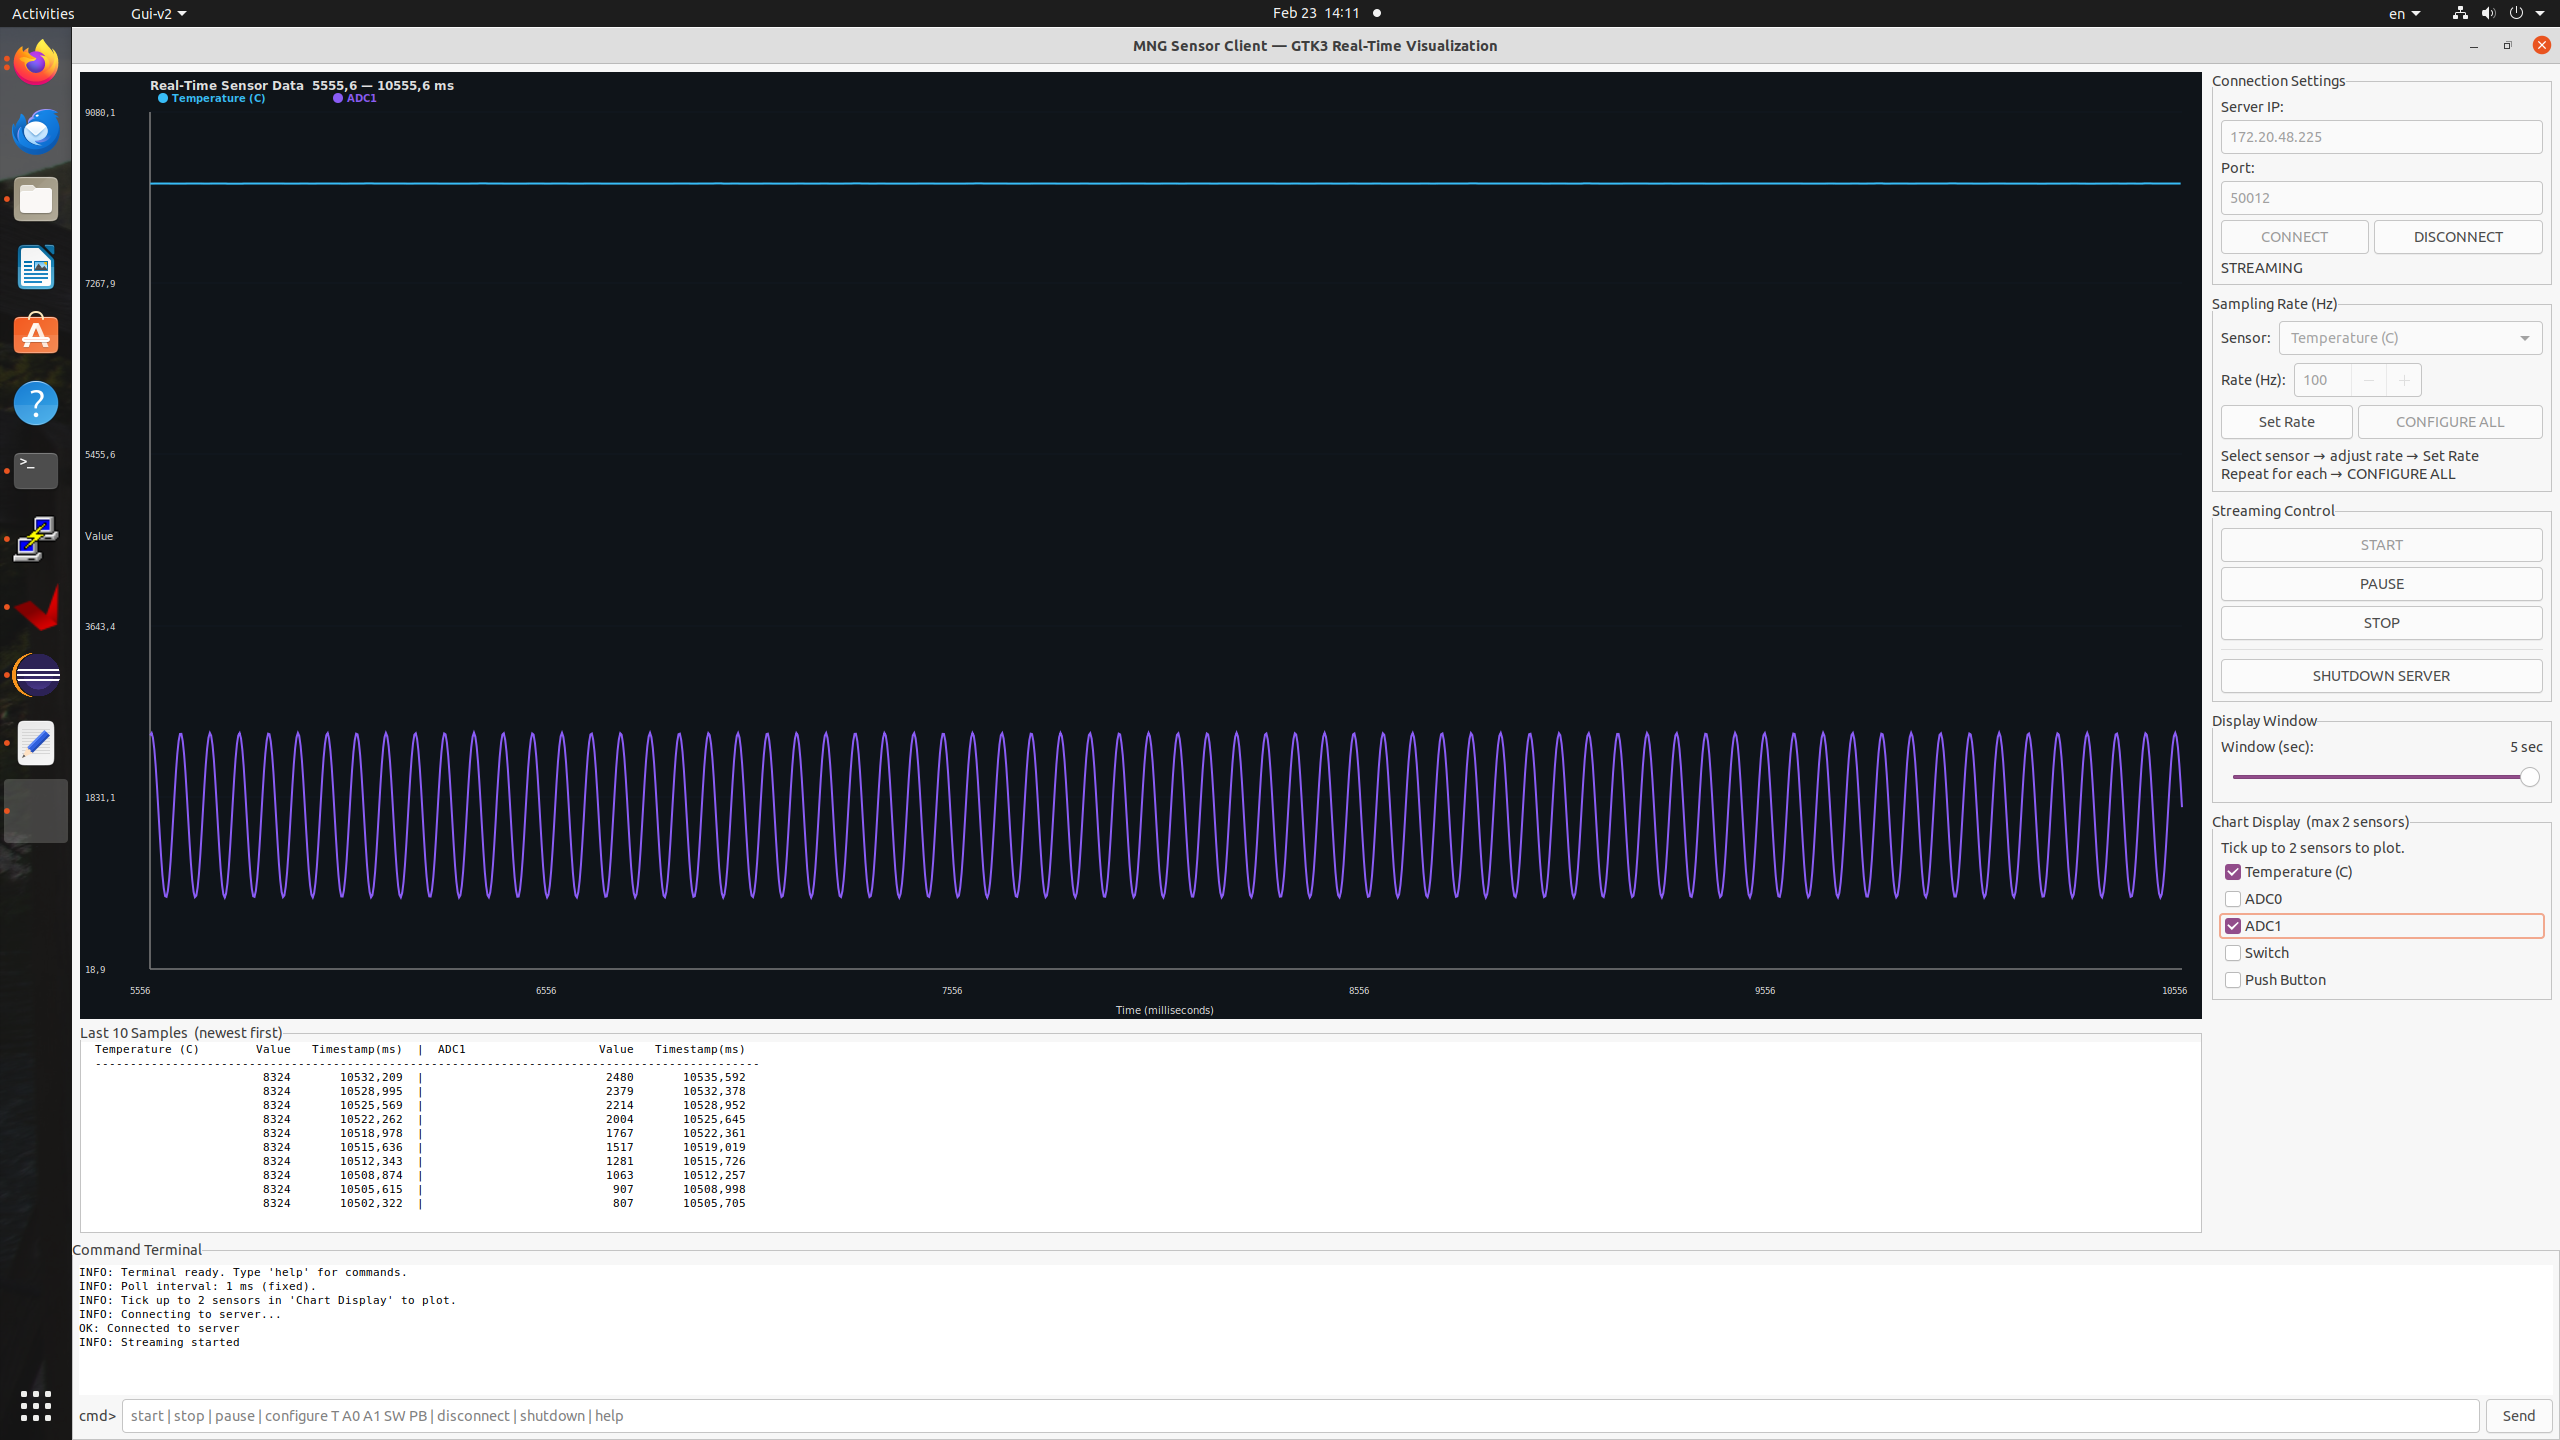
\includegraphics[scale = 0.29]{media/sc3.png}
    \caption{MNG Sensor Client main window overview.}
    \label{fig:gui_overview}
\end{figure}
\end{landscape}
The waveform chart renders up to two sensor signals simultaneously, each
distinguished by a unique colour. The horizontal axis represents elapsed time
in milliseconds, and the vertical axis displays the corresponding raw sensor
values. The visible time window is adjustable through a slider in the control
panel, ranging from 1 to 5 seconds, allowing the user to inspect both
short-term signal behaviour and longer acquisition trends.


\begin{figure}[H]
    \centering
        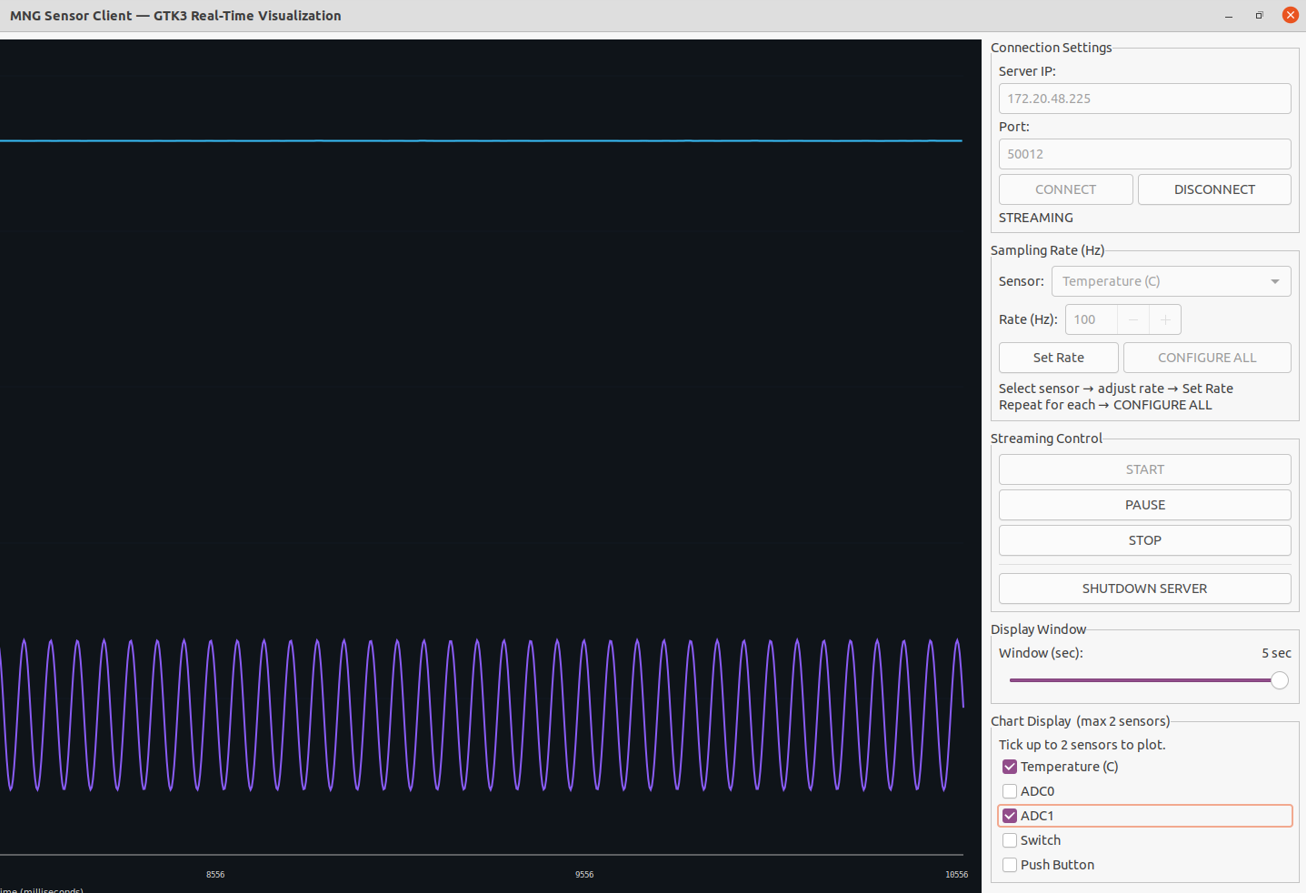
\includegraphics[width=0.8\textwidth]{media/panel_mahdi.png}
        \caption{GUI in active streaming session.}
        \label{fig:gui_streaming}
\end{figure}

\begin{figure}[H]
    \centering
    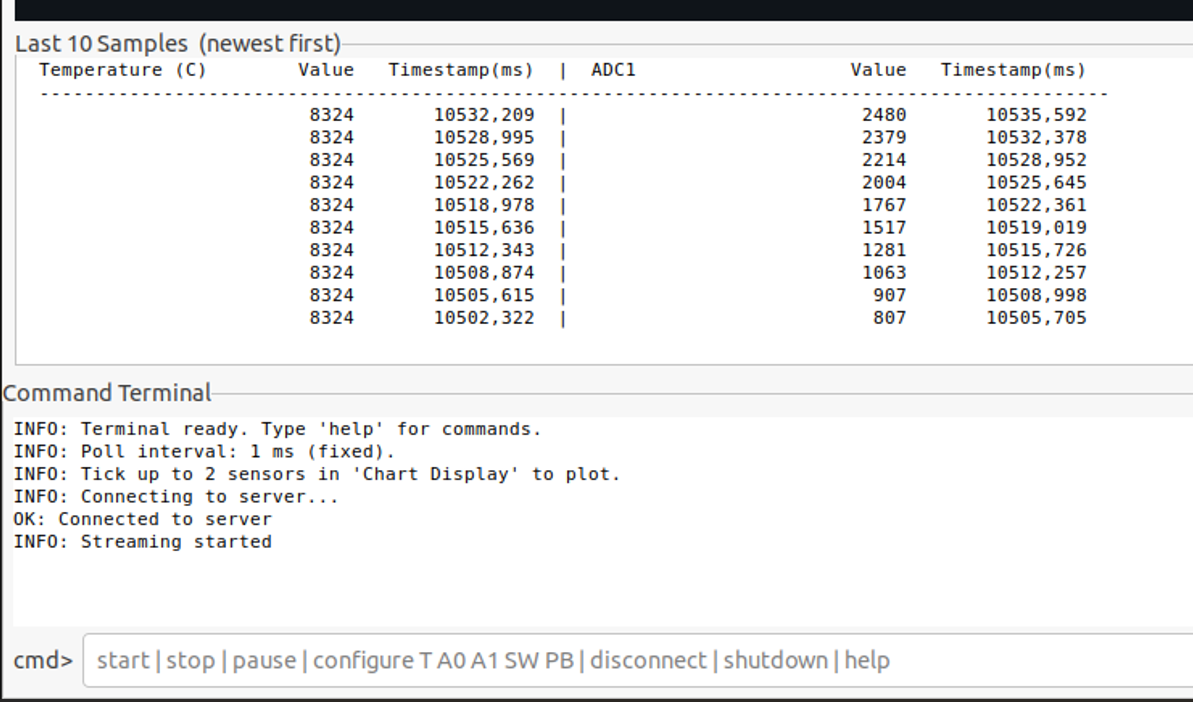
\includegraphics[width=0.8\textwidth]{media/terminal_mahdi.png}
    \caption{Embedded command terminal showing session log}
    \label{fig:gui_terminal}
\end{figure}



As shown in Figure~\ref{fig:gui_streaming}, during an active streaming session
the START button is disabled and the PAUSE and STOP buttons become available,
reflecting the current operational state enforced by the
\texttt{update\_button\_states()} function. The status label at the top of the
control panel updates in real time to indicate the current state, displaying
\texttt{STREAMING}, \texttt{PAUSED}, or \texttt{Connected - Ready} as
appropriate.

The embedded command terminal, shown in Figure~\ref{fig:gui_terminal}, provides
a text-based interface at the bottom of the window through which the user can
issue control commands directly. All session events --- including connection
establishment, configuration changes, streaming state transitions, and error
conditions are logged to the terminal with appropriate prefixes
(\texttt{INFO}, \texttt{OK}, \texttt{WARN}, \texttt{ERROR}), giving the user a
complete chronological record of the session activity.




%\section{UI layout and user Interaction}
%\subsection{Application Context and Initialization}
%\subsection{Callbacks and periodic refresh}

